\chapter{الكهرباء الساكنة: المجال وقانون غاوس}\label{ch:b1:electrostatics-gauss}

افرك منطادًا بكنزة صوفية يلتصق بالجدار؛ ومشّط شعرًا جافًّا
يحرف المشط خيطًا رفيعًا من الماء. ووراء الأمرين القوة بين
الشحن الكهربائية الساكنة، وهي \omterm{thm:b1:electrostatics-gauss:coulomb}{قانون كولوم} --- قانون تربيعي عكسي
كالثقالة، لكنه أقوى $10^{36}$ مرة بين بروتونين، وهو ذو
إشارتين، فتكون المادة متعادلة بدقة مذهلة وتكون
الآثار المتبقية ما نسمّيه الكيمياء والمواد والبرق.
ويبني هذا الفصل المفهوم الذي يجعل القانون قابلًا للمعالجة،
وهو \omterm{def:b1:electrostatics-gauss:field}{المجال الكهربائي}، ويبيّن كيف يُقرأ مجال من تناظراته،
ويشتقّ المبرهنة الوحيدة التي تحسب مجالات التوزيعات
المتناظرة في ثلاثة أسطر: هي \omterm{thm:b1:electrostatics-gauss:gauss}{قانون غاوس}. ويأتي توأمه
الثقالي مجانًا في الآخر.

\begin{omfigure}
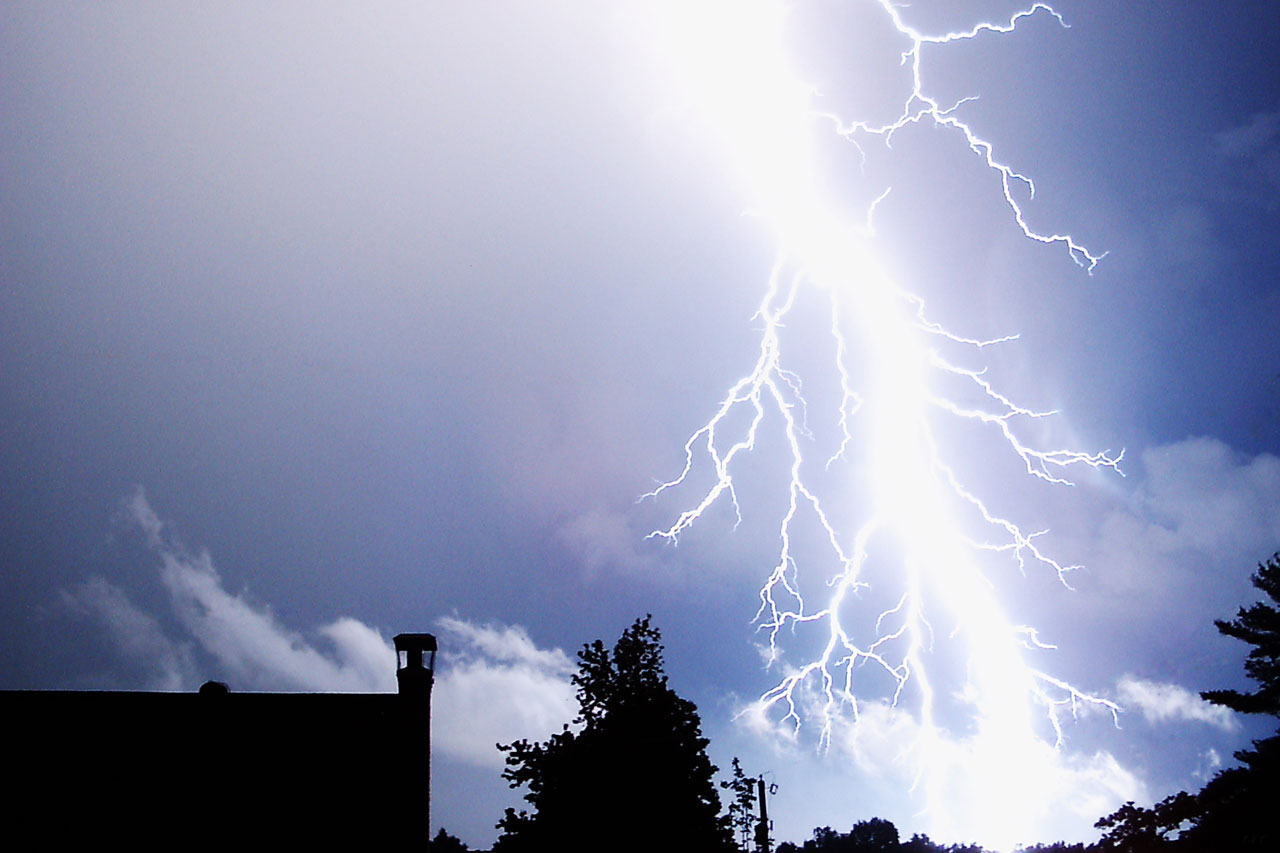
\includegraphics[width=0.50\linewidth]{images/book3/lightning-strike.jpg}

{\small برق من السحابة إلى الأرض: عشرات الكولومات تنزل في بضع ضربات شدة كلٍّ منها مئة كيلوأمبير --- وهي الأرض الكهربائية في مسألة نهاية الأسبوع.}
\end{omfigure}

\section{الشحن وقانون كولوم}

\begin{definition}[الشحنة الكهربائية]\label{def:b1:electrostatics-gauss:charge}
\index{شحنة كهربائية}\index{شحنة أولية}\index{كثافة الشحنة}
\emph{الشحنة الكهربائية} $q$ (بالكولوم، \unit{C}) خاصية للمادة
ذات إشارتين؛ وهي محفوظة (فالشحنة الكلية لجملة معزولة
لا تتغير أبدًا) ومكمّاة بمضاعفات \emph{الشحنة الأولية}
$e = \qty{1.602e-19}{C}$ (فللبروتون $+e$ وللإلكترون $-e$). ويُوصَف
التوزيع العياني بمقدار هو \emph{كثافة الشحنة}: خطية $\lambda$
(\unit{C/m})، أو سطحية $\sigma$ (\unit{C/m^2})، أو حجمية $\rho$
(\unit{C/m^3})، بحيث يحمل عنصر صغير $\dd q = \lambda\,\dd l$
أو $\sigma\,\dd S$ أو $\rho\,\dd\tau$.
\end{definition}

\begin{theorem}[قانون كولوم]\label{thm:b1:electrostatics-gauss:coulomb}
\index{قانون كولوم}\index{سماحية الخلاء}
شحنتان نقطيتان $q_1$ عند $M_1$ و $q_2$ عند $M_2$ ساكنتان في الخلاء
تؤثر كلٌّ منهما في الأخرى بالقوى
\[
\vect F_{1 \to 2} = \frac{q_1q_2}{4\pi\varepsilon_0\,r^2}\,\vect e_{12} = -\vect F_{2 \to 1},
\qquad r = M_1M_2,\quad \vect e_{12} = \frac{\vect{M_1M_2}}{r},
\]
وهي تنافرية بين شحنتين متماثلتَي الإشارة وتجاذبية بين مختلفتَيها، مع
\emph{\omterm{thm:b1:electrostatics-gauss:coulomb}{سماحية الخلاء}} $\varepsilon_0 = \qty{8.854e-12}{F/m}$، أي
$1/4\pi\varepsilon_0 = \qty{8.99e9}{N.m^2/C^2}$. وتتجمع القوى الآتية من عدة شحن
(وهو التراكب).
\end{theorem}
\admitted

\begin{example}[كم هي قوية]\label{ex:b1:electrostatics-gauss:strong}
بروتونان يفترقان \qty{1}{fm} يتنافران بالقوة $8.99 \times 10^9 \times (1.6 \times
10^{-19})^2/10^{-30} = \qty{230}{N}$ --- أي ثقل طفل، بين
جسيمين كتلة كلٍّ منهما $10^{-27}$~كيلوغرام؛ أما تجاذبهما الثقالي
فأصغر $10^{36}$ مرة. وغرامان من الإلكترونات في طرف غرفة
والبروتونات المقابلة لها في الطرف الآخر يتجاذبان بقوة $10^{25}$~نيوتن.
والمادة متعادلة لأنها لا تملك خيارًا: فأيّ اختلال تصحّحه
قوى لا يقاومها بناء.
\end{example}

\section{المجال الكهربائي}

\begin{definition}[مجال الكهرباء الساكنة]\label{def:b1:electrostatics-gauss:field}
\index{مجال كهربائي}\index{خط المجال}
يُحدث توزيع من شحن ساكنة عند كل نقطة $M$ من الفضاء
\emph{مجالًا كهربائيًّا} $\vect E(M)$، يُعرَّف بالقوة التي يؤثر بها في
شحنة اختبار $q$ توضع عند $M$: $\vect F = q\vect E(M)$ (بوحدة \unit{V/m} $=$
\unit{N/C}). وتُحدث شحنة نقطية $q_1$ عند $O$ المجالَ
\[
\vect E(M) = \frac{q_1}{4\pi\varepsilon_0 r^2}\,\vect e_r , \qquad r = OM ,
\]
وهو قطري، إلى الخارج إن كان $q_1 > 0$؛ ويُحدث توزيعٌ المجموعَ المتجهي
لمجالات عناصره. و\emph{خط المجال} منحنٍ يماسّ عند كل
نقطة المتجهةَ $\vect E$، ويُوجَّه في جهته.
\end{definition}

\begin{proposition}[قراءة خريطة مجال]\label{prop:b1:electrostatics-gauss:lines}
تغادر \omterm{def:b1:electrostatics-gauss:field}{خطوط المجال} الشحن الموجبة وتنتهي على السالبة (أو عند
اللانهاية)؛ ولا تتقاطع أبدًا (فالمجال وحيد القيمة)، وتتزاحم
حيث يكون المجال قويًّا. وحين تحضر شحنتان يتناسب عدد
الخطوط المرسومة من كلٍّ منهما مع شحنتها.
\end{proposition}

\begin{omfigure}
\begin{tikzpicture}[font=\small, x=1cm, y=1cm, >=Stealth]
  % dipole: arcs through (-1,0) and (1,0), centre (0,c)
  \begin{scope}[scale=1.4]
    \foreach \c in {0.1, 0.55, 1.6} {
      \draw[omDef, thick, postaction={decorate, decoration={markings, mark=at position 0.5 with {\arrow{>}}}}]
        let \n1 = {sqrt(1+\c*\c)} in
        (-1,0) arc[start angle={180+atan2(\c,1)}, end angle={360-atan2(\c,1)}, radius=\n1 cm];
      \draw[omDef, thick, postaction={decorate, decoration={markings, mark=at position 0.5 with {\arrow{>}}}}]
        let \n1 = {sqrt(1+\c*\c)} in
        (-1,0) arc[start angle={180-atan2(\c,1)}, end angle={atan2(\c,1)}, radius=\n1 cm];
    }
    \draw[omDef, thick, postaction={decorate, decoration={markings, mark=at position 0.5 with {\arrow{>}}}}] (-1,0) -- (1,0);
    \draw[omDef, thick, postaction={decorate, decoration={markings, mark=at position 0.6 with {\arrow{>}}}}] (-2.6,0) -- (-1,0);
    \draw[omDef, thick, postaction={decorate, decoration={markings, mark=at position 0.4 with {\arrow{>}}}}] (1,0) -- (2.6,0);
    \fill[omThm] (-1,0) circle (3pt) node[below left] {$+q$};
    \fill[omDef] (1,0) circle (3pt) node[below right] {$-q$};
  \end{scope}
  % two like charges
  \begin{scope}[xshift=7.9cm, fl/.style={omThm, thick, postaction={decorate, decoration={markings, mark=at position 0.55 with {\arrow{>}}}}}]
    \foreach \s in {1,-1} {
      % left charge at (-1,0), right charge at (1,0); \s mirrors up/down
      \draw[fl] (-1,0) -- (-3.4,0);
      \draw[fl] (1,0) -- (3.4,0);
      \draw[fl] (-1,0) .. controls (-2.2,{1.2*\s}) .. (-3.2,{2.0*\s});
      \draw[fl] (1,0) .. controls (2.2,{1.2*\s}) .. (3.2,{2.0*\s});
      \draw[fl] (-1,0) .. controls (-1.1,{1.3*\s}) .. (-1.6,{2.9*\s});
      \draw[fl] (1,0) .. controls (1.1,{1.3*\s}) .. (1.6,{2.9*\s});
      \draw[fl] (-1,0) .. controls (-0.2,{0.7*\s}) and (-0.1,{1.6*\s}) .. (-0.3,{2.9*\s});
      \draw[fl] (1,0) .. controls (0.2,{0.7*\s}) and (0.1,{1.6*\s}) .. (0.3,{2.9*\s});
    }
    \draw[fl] (-1,0) -- (-0.08,0);
    \draw[fl] (1,0) -- (0.08,0);
    \fill[omThm] (-1,0) circle (3pt) node[below left] {$+q$};
    \fill[omThm] (1,0) circle (3pt) node[below right] {$+q$};
    \fill (0,0) circle (1.2pt) node[below, font=\footnotesize, yshift=-2pt] {$\vect E = \vect 0$};
  \end{scope}
\end{tikzpicture}

{\small خطوط مجال شحنتين متعاكستين (على اليمين) وشحنتين
موجبتين متساويتين (على اليسار). فالخطوط تبدأ على $+$ وتنتهي على $-$ أو عند
اللانهاية؛ وعلى اليسار يتنافر بعضها مع بعض وينعدم المجال عند
منتصف المسافة، حيث لا يمرّ أيّ خط.}
\end{omfigure}

\begin{example}[حلقة وقطعة بالجمع المباشر]\label{ex:b1:electrostatics-gauss:ring}
على محور حلقة نصف قطرها $R$ تحمل $Q$ بانتظام، وعلى مسافة
$z$ من مركزها، يسهم كل عنصر $\dd q$ بالمقدار $\dd q/4\pi\varepsilon_0(R^2 +
z^2)$ على امتداد المستقيم الواصل بينه وبين $M$؛ وتتلاشى المركّبات العمودية
على المحور مثنى مثنى وتتجمع المحورية بالعامل
$z/\sqrt{R^2 + z^2}$:
\[
E_z = \frac{Qz}{4\pi\varepsilon_0(R^2 + z^2)^{3/2}} ,
\]
وهو معدوم عند المركز، وأعظمي عند $z = R/\sqrt2$، ويساوي $Q/4\pi\varepsilon_0z^2$ في
البعد. والقرص المشحون بانتظام كومة من الحلقات (\cref{pb:b1:electrostatics-gauss:1}).
والجمع المباشر ينفع كلما سمحت الهندسة بحساب التكامل؛ وبقية
الفصل في تجنّبه.
\end{example}

\section{التناظرات وعدم التغيّر}

\begin{proposition}[مبدأ التناظر]\label{prop:b1:electrostatics-gauss:symmetry}
\index{تناظر (مجال)}\index{مستوي تناظر}\index{مستوي تناظر عكسي}
للمجال تناظرات منابعه. فإذا كان مستوٍ $\Pi$ \emph{\omterm{prop:b1:electrostatics-gauss:symmetry}{مستوي تناظر}}
لتوزيع الشحن (أي إن صورة التوزيع في المرآة هي هو)،
كان المجال عند كل نقطة من $\Pi$ واقعًا \emph{في} $\Pi$؛ وإذا كان $\Pi$
\emph{\omterm{prop:b1:electrostatics-gauss:symmetry}{مستوي تناظر عكسي}} (أي إن صورة المرآة هي التوزيع
وقد عُكست إشارات شحنه كلها)، كان المجال عند نقاط $\Pi$
\emph{عموديًّا} على $\Pi$. وإذا كان التوزيع لا يتغير بانسحاب أو بدوران،
لم يتغير المجال كذلك: فلا تتوقف مركّباته على الإحداثي الموافق.
\end{proposition}

\begin{proof}
$\vect E$ مجموع حدود $\dd q\,\vect e/4\pi\varepsilon_0r^2$؛ وصورة المجموع في
المرآة هي مجموع الصور، وصورة مجال
توزيع هي مجال التوزيع الصورة (فالمتجهة المبنية
من المواضع والشحن تتحول كما تتحول المواضع). وعلى
\omterm{prop:b1:electrostatics-gauss:symmetry}{مستوي تناظر} يساوي المجال صورته في المرآة، فيقع في
المستوي؛ وعلى \omterm{prop:b1:electrostatics-gauss:symmetry}{مستوي تناظر عكسي} يساوي معاكس صورته،
فيكون ناظميًّا عليه. وعدم التغيّر هو الحجة نفسها مع
انسحاب أو دوران.
\end{proof}

\begin{method}[إيجاد شكل المجال قبل حسابه]\label{meth:b1:electrostatics-gauss:symmetry}
من أجل النقطة $M$ التي يُطلَب المجال عندها: (1) اذكر مستويات
تناظر المنابع التي تحوي $M$ --- فالمجال يقع على
تقاطعها؛ ومستويان كهذان يعيّنان الجهة. (2) واذكر
عدم التغيّرات --- فهي تقول على أيّ إحداثيات يتوقف $\vect E$. وهكذا يعطي
سلك لانهائي مشحون بانتظام $\vect E = E(r)\,\vect e_r$ في
\omterm{def:b1:point-kinematics:cylindrical}{الإحداثيات الأسطوانية}، وتعطي كرة $\vect E = E(r)\,\vect e_r$ في
الكروية، ويعطي مستوٍ لانهائي $\vect E = E(z)\,\vect e_z$ مع $E(-z) = -E(z)$.
وعندئذ فقط احسب.
\end{method}

\begin{omfigure}
\begin{tikzpicture}[font=\small, x=1cm, y=1cm, >=Stealth]
  % sphere
  \begin{scope}
    \draw[omDef, fill=omDef!15] (0,0) circle (0.9);
    \draw[dashed] (0,0) circle (1.8);
    \foreach \a in {0,45,...,315} \draw[omThm, thick, ->] (\a:1.8) -- ++(\a:0.6);
    \node[font=\footnotesize] at (0,-2.75) {$\vect E = E(r)\,\vect e_r$};
    \node[font=\footnotesize, omDef] at (0,0) {$Q$};
  \end{scope}
  % cylinder / wire
  \begin{scope}[xshift=5.2cm]
    \draw[omDef, very thick] (0,-2.2) -- (0,2.2) node[above, font=\footnotesize] {$\lambda$};
    \draw[dashed] (-1.1,-1.6) rectangle (1.1,1.6);
    \draw[dashed] (0,1.6) ellipse (1.1 and 0.28);
    \draw[dashed] (0,-1.6) ellipse (1.1 and 0.28);
    \foreach \y in {-1.0,-0.3,0.4,1.1} {\draw[omThm, thick, ->] (1.1,\y) -- ++(0.6,0); \draw[omThm, thick, ->] (-1.1,\y) -- ++(-0.6,0);}
    \node[font=\footnotesize] at (0,-2.75) {$\vect E = E(r)\,\vect e_r$ (أسطوانية)};
  \end{scope}
  % plane
  \begin{scope}[xshift=10.4cm]
    \draw[omDef, fill=omDef!25] (-1.8,-0.25) -- (1.8,-0.25) -- (2.2,0.25) -- (-1.4,0.25) -- cycle;
    \node[omDef, font=\footnotesize] at (1.9,-0.45) {$\sigma$};
    \draw[dashed] (-0.5,-1.4) rectangle (0.5,1.4);
    \foreach \x in {-1.2,0,1.2} {\draw[omThm, thick, ->] (\x,0.35) -- ++(0,0.9); \draw[omThm, thick, ->] (\x,-0.35) -- ++(0,-0.9);}
    \node[font=\footnotesize] at (0,-2.75) {$\vect E = E(z)\,\vect e_z$، فردي في $z$};
  \end{scope}
\end{tikzpicture}

{\small التوزيعات المتناظرة الثلاثة في هذا الفصل، وسطوح
غاوس (المتقطعة) الملائمة لها: كرة متحدة المركز، وأسطوانة
متحدة المحور، وعلبة مسطّحة تعتلي المستوي. وعلى كلٍّ منها يكون المجال
إما ناظميًّا ومنتظم الطويلة وإما مماسيًّا.}
\end{omfigure}

\section{التدفق وقانون غاوس}

\begin{definition}[تدفق المجال]\label{def:b1:electrostatics-gauss:flux}
\index{تدفق المجال الكهربائي}
اقطع سطحًا $S$ إلى عناصر صغيرة مساحة كلٍّ منها $\dd S$، ولكلٍّ ناظم
واحدي $\vect n$ (وهو الناظم الخارجي في سطح مغلق). ويكون
\emph{تدفق} $\vect E$ عبر $S$ هو المجموع
\[
\Phi = \sum \vect E\cdot\vect n\,\dd S = \sum E_n\,\dd S \qquad (\unit{V.m}):
\]
أي المركّبة الناظمية للمجال موزونةً بالمساحة --- وهو ``عدد \omterm{def:b1:electrostatics-gauss:field}{خطوط
المجال}'' التي تعبر $S$، محسوبةً موجبةً حين تعبر في جهة
$\vect n$.
\end{definition}

\begin{theorem}[قانون غاوس]\label{thm:b1:electrostatics-gauss:gauss}
\index{قانون غاوس}
\omterm{def:b1:electrostatics-gauss:flux}{تدفق} مجال الكهرباء الساكنة عبر أيّ سطح مغلق $S$
يساوي الشحنة الكلية التي يحصرها $S$ مقسومةً على $\varepsilon_0$:
\[
\Phi_{\text{الخارج}} = \frac{Q_{\text{الداخل}}}{\varepsilon_0} .
\]
ولا تسهم الشحن الواقعة خارج $S$ في \omterm{def:b1:electrostatics-gauss:flux}{التدفق} بشيء (فخطوطها تدخل
ثم تخرج من جديد).
\end{theorem}

\begin{proof}
من أجل شحنة نقطية $q$ في مركز كرة نصف قطرها $r$:
يكون $\vect E$ قطريًّا، طويلته $q/4\pi\varepsilon_0r^2$ في كل موضع من
الكرة، ومنه $\Phi = E \times 4\pi r^2 = q/\varepsilon_0$ --- وهو مستقل عن $r$،
لأن المجال يتناقص بنسبة $1/r^2$ تمامًا كما تتزايد المساحة. أما أن
الأمر نفسه يصحّ من أجل أيّ سطح مغلق حول $q$ (إذ لا يتوقف \omterm{def:b1:electrostatics-gauss:flux}{التدفق} عبر
عنصر سطحي إلا على الزاوية المجسمة التي يقابلها من $q$)،
وأن شحنة خارجية تعطي صفرًا (لأنها تقابل كل زاوية مجسمة مرتين
بإشارتين متعاكستين)، وأن تدفقات عدة شحن تتجمع، فمسلَّم به
هنا؛ والبرهان التامّ في مجلد السنة الثانية.
\end{proof}

\begin{method}[استعمال قانون غاوس]\label{meth:b1:electrostatics-gauss:gauss}
(1) اكتب من التناظرات شكل $\vect E$ (أي جهته والمتغير
الذي يتوقف عليه). (2) واختر \emph{سطح غاوس} مغلقًا
يمرّ بالنقطة $M$ ويكون $\vect E$ في كل موضع منه إما ناظميًّا
بالطويلة $E(M)$ نفسها وإما مماسيًّا: فيكون \omterm{def:b1:electrostatics-gauss:flux}{التدفق} عندئذ $E(M)$ مضروبًا في
مساحة الجزء الناظمي. (3) وعُدّ الشحنة في الداخل. (4) وحُلّ لإيجاد
$E(M)$. وهو ينفع من أجل الكرات والأسطوانات اللانهائية والمستويات اللانهائية
--- ولا ينفع لغيرها بلا أدوات إضافية.
\end{method}

\begin{proposition}[المجالات الكلاسيكية الثلاثة]\label{prop:b1:electrostatics-gauss:three}
\index{مجال كرة مشحونة}\index{مجال سلك مشحون}\index{مجال مستوٍ مشحون}
\begin{enumerate}
  \item كرة نصف قطرها $R$ وشحنتها $Q$ موزعة بانتظام في
        حجمها: $E(r) = \dfrac{Q}{4\pi\varepsilon_0r^2}$ في الخارج ($r > R$) ---
        كأن الشحنة كلها في المركز --- ويكون $E(r) =
        \dfrac{Qr}{4\pi\varepsilon_0R^3}$ في الداخل، متزايدًا خطيًّا من الصفر؛
        وهو متصل عند $r = R$. أما إذا كانت الشحنة على السطح وحده
        فالمجال في الداخل معدوم.
  \item سلك لانهائي شحنته الخطية $\lambda$: $E(r) =
        \dfrac{\lambda}{2\pi\varepsilon_0 r}$، وهو قطري.
  \item مستوٍ لانهائي شحنته السطحية $\sigma$: $E = \dfrac{\sigma}{2\varepsilon_0}$
        من كل جهة، ناظمي على المستوي، مبتعدًا عنه إن كانت
        $\sigma > 0$، و\emph{مستقل عن المسافة}. وتقفز المركّبة الناظمية
        عبر المستوي بمقدار $\sigma/\varepsilon_0$.
\end{enumerate}
\end{proposition}

\begin{proof}
(1) كرة نصف قطرها $r$: \omterm{def:b1:electrostatics-gauss:flux}{التدفق} $4\pi r^2E(r)$؛ والشحنة في الداخل $Q$ إن كان
$r > R$، و $Q(r/R)^3$ إن كان $r < R$. (2) أسطوانة نصف قطرها $r$ وطولها $h$:
\omterm{def:b1:electrostatics-gauss:flux}{التدفق} عبر السطح الجانبي $2\pi rh\,E(r)$، ولا شيء عبر القاعدتين
(فالمجال مماسي)؛ والشحنة $\lambda h$. (3) علبة مسطّحة مقطعها $S$
تعتلي المستوي: \omterm{def:b1:electrostatics-gauss:flux}{التدفق} $2SE$ عبر القاعدتين (فالمجال فردي
في $z$، فتُحسبان معًا موجبتين)، ولا شيء عبر الجانب؛ والشحنة
$\sigma S$.
\end{proof}

\begin{omfigure}
\begin{tikzpicture}
\begin{axis}[omaxis, axis x line=bottom, axis y line=left, width=10cm, height=5.6cm,
    xlabel={$r/R$}, ylabel={$E$ (بوحدات $Q/4\pi\varepsilon_0R^2$)},
    xlabel style={at={(axis description cs:0.5,-0.1)}, anchor=north},
    xmin=0, xmax=4, ymin=0, ymax=1.3, xtick={1,2,3}, ytick={0.5,1}, samples=80]
  \addplot[omDef, very thick, domain=0:1] {x} node[pos=0.85, above left, font=\footnotesize] {حجمية: $\propto r$};
  \addplot[omDef, very thick, domain=1:4] {1/x^2} node[pos=0.35, above right, font=\footnotesize] {$\propto 1/r^2$};
  \addplot[omThm, thick, dashed] coordinates {(0,0) (1,0)};
  \addplot[omThm, thick, dashed] coordinates {(1,0) (1,1)};
  \node[omThm, font=\footnotesize, anchor=west] at (axis cs:1.08,0.08) {سطحية: $0$ في الداخل};
\end{axis}
\end{tikzpicture}

{\small \omterm{prop:b1:electrostatics-gauss:three}{مجال كرة مشحونة} بدلالة البعد عن مركزها:
خطي في الداخل وبالمقدار $1/r^2$ في الخارج حين تملأ الشحنة الحجم
(الخط المتصل)؛ ومعدوم في الداخل وهو هو في الخارج حين تستقر على السطح
(الخط المتقطع). وفي الخارج لا شيء يميّز الكرة من شحنة نقطية
في مركزها.}
\end{omfigure}

\begin{example}[مستويان: المكثف المستوي]\label{ex:b1:electrostatics-gauss:twoplanes}
\index{مكثف مستوٍ!المجال}
مستويان متوازيان يحملان $+\sigma$ و $-\sigma$: يُحدث كلٌّ منهما
$\sigma/2\varepsilon_0$ مبتعدًا عنه (ومتجهًا نحوه في السالب).
وبين المستويين يتجمع المجالان فيعطيان $\sigma/\varepsilon_0$، موجَّهًا من
$+$ إلى $-$؛ وفي الخارج يتلاشيان. ومع $\sigma = \qty{1}{\micro C/m^2}$ يكون $E =
10^{-6}/8.85 \times 10^{-12} = \qty{1.1e5}{V/m}$ بينهما، ومعدومًا في الخارج:
فمجال مكثف مشحون محصور في فجوته
(\cref{ch:b1:potential-capacitors}).
\end{example}

\begin{omfigure}
\begin{tikzpicture}[font=\small, x=1cm, y=1cm, >=Stealth]
  \draw[omThm, very thick] (-0.8,-2) -- (-0.8,2) node[above] {$+\sigma$};
  \draw[omDef, very thick] (0.8,-2) -- (0.8,2) node[above] {$-\sigma$};
  % field of + plane (red), of - plane (blue), resultant (black)
  \foreach \y in {-1.4,-0.7,0,0.7,1.4} {
    \draw[omThm, ->] (-0.8,\y) -- ++(0.55,0);
    \draw[omThm, ->] (-0.8,\y) -- ++(-0.55,0);
    \draw[omDef, ->] (0.8,\y) -- ++(-0.55,0);
    \draw[omDef, ->] (0.8,\y) -- ++(0.55,0);
  }
  \node[omThm, font=\footnotesize, anchor=east] at (-1.0,-2.4) {$+\sigma$ وحده: $\sigma/2\varepsilon_0$};
  \node[omDef, font=\footnotesize, anchor=west] at (1.0,-2.4) {$-\sigma$ وحده: $\sigma/2\varepsilon_0$};
  \begin{scope}[xshift=7.2cm]
    \draw[omThm, very thick] (-0.8,-2) -- (-0.8,2) node[above] {$+\sigma$};
    \draw[omDef, very thick] (0.8,-2) -- (0.8,2) node[above] {$-\sigma$};
    \foreach \y in {-1.4,-0.7,0,0.7,1.4} \draw[black, very thick, ->] (-0.75,\y) -- (0.7,\y);
    \node[font=\footnotesize] at (0,-2.4) {المجموع: $\sigma/\varepsilon_0$ بينهما، و $0$ في الخارج};
  \end{scope}
\end{tikzpicture}

{\small التراكب من أجل صفيحتين متعاكستين. على اليمين: المجالان المنتظمان
لكل صفيحة وحدها (بالأحمر من الموجبة، وبالأزرق نحو السالبة).
وعلى اليسار: مجموعهما، $\sigma/\varepsilon_0$ في الفجوة وصفر فيما عداها.}
\end{omfigure}

\section{المماثلة الثقالية}

\begin{proposition}[قانون غاوس للثقالة]\label{prop:b1:electrostatics-gauss:gravity}
\index{قانون غاوس!للثقالة}\index{مجال ثقالي}
لقانون نيوتن $\vect F = -Gm_1m_2\,\vect e_{12}/r^2$ شكل
\omterm{thm:b1:electrostatics-gauss:coulomb}{قانون كولوم} مع $q \to m$ و $1/4\pi\varepsilon_0 \to -G$. ومن ثمّ يخضع
\omterm{prop:b1:electrostatics-gauss:gravity}{المجال الثقالي} $\vect g$ (وهو القوة لواحدة الكتلة) لقواعد التناظر نفسها
ويحقق
\[
\Phi_{\text{الخارج}}(\vect g) = -4\pi G\,M_{\text{الداخل}} .
\]
وعلى الخصوص، يجذب جسم متناظر كرويًّا النقاطَ الخارجية كأن
كتلته في مركزه، ويكون المجال داخل كرة منتظمة
نصف قطرها $R$ وكتلتها $M$ هو $g(r) = GMr/R^3$، أي خطيًّا في $r$.
\end{proposition}

\begin{proof}
استبدل بالمقدار $Q/\varepsilon_0$ المقدارَ $-4\pi GM$ في برهان
\cref{prop:b1:electrostatics-gauss:three}؛ وتقول الإشارة السالبة إن \omterm{def:b1:electrostatics-gauss:flux}{التدفق}
داخل (فالثقالة جاذبة).
\end{proof}

\begin{example}[داخل الأرض]\label{ex:b1:electrostatics-gauss:earth}
لو كانت الأرض منتظمة لهبطت $g$ خطيًّا من \qty{9.8}{m/s^2} عند
السطح إلى الصفر عند المركز؛ ولاهتزّ حجر يُسقَط في نفق يخترق
الكوكب اهتزازًا توافقيًّا دوره $2\pi\sqrt{R/g} =
\qty{84}{min}$ --- وهو دور قمر صناعي ملامس. أما الأرض الحقيقية فلها
لبّ كثيف، و $g$ فيها \emph{ترتفع} فعلًا إلى \qty{10.7}{m/s^2} عند
حدّ اللبّ والوشاح قبل أن تهبط (\cref{pb:b1:electrostatics-gauss:1}).
وقد احتاج نيوتن إلى مبرهنة القشرة ليطبّق قانونه على الكواكب؛ أما \omterm{thm:b1:electrostatics-gauss:gauss}{قانون
غاوس} فيعطيها في سطر.
\end{example}

\section{تمارين}

\begin{exercise}[$\star$]\label{exo:b1:electrostatics-gauss:1}
أوجد القوة الكهربائية والقوة الثقالية بين بروتونين يفترقان
\qty{2.0}{fm}؛ ونسبتهما. ولماذا تتماسك النوى إذن؟
\end{exercise}

\begin{exercise}[$\star$]\label{exo:b1:electrostatics-gauss:2}
المجال على بعد \qty{1.0}{m} من شحنة نقطية \qty{1.0}{\micro C}. ويحمل سطح
الأرض مجالًا قدره \qty{100}{V/m} متجهًا نحو الأسفل: أوجد إشارة شحنة
الأرض وقيمتها، بمعاملتها كرةً نصف قطرها \qty{6370}{km}.
\end{exercise}

\begin{exercise}[$\star$]\label{exo:b1:electrostatics-gauss:3}
شحنتان $+q$ عند $x = \pm a$ على المحور $x$. أوجد المجال على المحور $x$
من أجل $|x| > a$ وعلى المحور $y$؛ وبيّن أنه على المحور $y$ يكون $E_y$
أعظميًّا عند $y = a/\sqrt2$. وارسم الخطوط قرب المبدأ.
\end{exercise}

\begin{exercise}[$\star$]\label{exo:b1:electrostatics-gauss:4}
شحنتان $+2q$ عند $x = 0$ و $-q$ عند $x = a$. أين ينعدم المجال على
المحور $x$؟ وكم خط مجال يغادر $+2q$ مقابل كل خط
يصل إلى $-q$، وإلى أين تذهب البقية؟
\end{exercise}

\begin{exercise}[$\star\star$]\label{exo:b1:electrostatics-gauss:5}
قرص نصف قطره $R$ يحمل $\sigma$ بانتظام. انطلاقًا من نتيجة الحلقة،
بيّن أن $E_z = \dfrac{\sigma}{2\varepsilon_0}\Bigl(1 - \dfrac{z}{\sqrt{z^2 +
R^2}}\Bigr)$ من أجل $z > 0$؛ وتحقّق من النهايتين $z \ll R$ و $z \gg R$.
\end{exercise}

\begin{exercise}[$\star\star$]\label{exo:b1:electrostatics-gauss:6}
نواة ذهب ($Z = 79$ و $R = \qty{7.0}{fm}$) بوصفها كرة مشحونة
بانتظام: أوجد المجال عند سطحها، وعند $R/2$، وعند \qty{1}{pm}. وقارنه
بمجال انهيار الهواء، وهو \qty{3e6}{V/m}.
\end{exercise}

\begin{exercise}[$\star\star$]\label{exo:b1:electrostatics-gauss:7}
مجال سلك لانهائي \omterm{thm:b1:electrostatics-gauss:gauss}{بقانون غاوس}. وناقل عالي التوتر نصف
قطره \qty{1.0}{cm}: أوجد الشحنة الخطية التي يبلغ عندها المجال على سطحه
قيمة الانهيار \qty{3e6}{V/m} (وهي بداية التفريغ الهالي). ثم المجال على بعد
\qty{5}{m} عندئذ.
\end{exercise}

\begin{exercise}[$\star\star$]\label{exo:b1:electrostatics-gauss:8}
صفيحتان متوازيتان مساحة كلٍّ منهما \qty{1.0}{m^2} تحملان $\pm\qty{1.0}{\micro C}$.
أوجد المجال بينهما؛ والقوة على إحدى الصفيحتين (فالمجال المؤثر فيها هو
مجال الصفيحة الأخرى وحدها --- ولماذا؟)؛ والضغط على الصفيحتين.
\end{exercise}

\begin{exercise}[$\star\star$]\label{exo:b1:electrostatics-gauss:9}
كبل محوري: ناقل داخلي نصف قطره $a$ يحمل $+\lambda$، وغلاف
خارجي نصف قطره $b$ يحمل $-\lambda$. أوجد المجال في المناطق الثلاث \omterm{thm:b1:electrostatics-gauss:gauss}{بقانون
غاوس}. ومع $a = \qty{0.5}{mm}$ و $b = \qty{2.5}{mm}$ و $\lambda = \qty{10}{nC/m}$:
أوجد المجال على سطح الناقل الداخلي.
\end{exercise}

\begin{exercise}[$\star\star\star$]\label{exo:b1:electrostatics-gauss:10}
قشرة كروية سميكة $R_1 < r < R_2$ تحمل $Q$ بانتظام في
حجمها. أوجد المجال في المناطق الثلاث؛ وتحقّق من الاتصال عند $R_1$ و
$R_2$؛ وأين يكون أعظميًّا؟ وارسم $E(r)$. وشحنة موجبة توضع
في التجويف: ما القوة التي تحسّها؟
\end{exercise}

\begin{exercise}[$\star\star\star$]\label{exo:b1:electrostatics-gauss:11}
\emph{الثقالة داخل الأرض.} اللبّ: نصف قطره \qty{3480}{km} وكثافته
\qty{11000}{kg/m^3}؛ والوشاح حتى \qty{6370}{km} وكثافته \qty{4500}{kg/m^3}.
(أ) أوجد كتلة اللبّ وكتلة الوشاح والكتلة الكلية (وقارنها بالقيمة \qty{5.97e24}{kg}).
(ب) و $g$ عند السطح وعند حدّ اللبّ والوشاح. (ج) وبيّن أن
$g$ تتزايد مع العمق في الوشاح إذا كانت كثافة الوشاح دون
$\tfrac23$ من متوسط كثافة ما تحته، وتحقّق من ذلك.
\end{exercise}

\begin{exercise}[$\star\star\star$]\label{exo:b1:electrostatics-gauss:12}
\emph{ذرة طومسون.} انمذج ذرة الهيدروجين كرةً موجبة
منتظمة شحنتها $+e$ ونصف قطرها $R = \qty{0.10}{nm}$ والإلكترون
حرّ في داخلها. (أ) أوجد القوة على الإلكترون على بعد $r$ من المركز.
(ب) وبيّن أنه يهتزّ اهتزازًا توافقيًّا واحسب التواتر
وطول موجة الضوء الذي كان ليصدره. (ج) وقارن مع
خطوط الهيدروجين فوق البنفسجية (\qty{122}{nm} وأقصر) وعلّق على
ما يصيبه النموذج وما يخطئ فيه (\cref{ch:b1:quantum-introduction}).
\end{exercise}

\section{مسألة: الأرض الكهربائية}

\begin{problem}[{مسألة نهاية الأسبوع --- مجال الطقس الصافي،
والسحابة الرعدية، وضربة البرق، وقانون غاوس مسلَّطًا على الثقالة}]
\label{pb:b1:electrostatics-gauss:1}
المعطيات: $\varepsilon_0 = \qty{8.85e-12}{F/m}$، و $1/4\pi\varepsilon_0 = \qty{8.99e9}{SI}$،
و $e = \qty{1.6e-19}{C}$، ونصف قطر الأرض $R_E = \qty{6.37e6}{m}$، ومساحة سطحها
$\qty{5.1e14}{m^2}$، و $G = \qty{6.67e-11}{SI}$، و $M_E = \qty{5.97e24}{kg}$.

\medskip
\noindent\textbf{الجزء I --- مجال الطقس الصافي.}
في الطقس الصافي يكون المجال عند الأرض $E_0 = \qty{100}{V/m}$،
متجهًا نحو \emph{الأسفل}.
\begin{enumerate}
  \item جهة القوة المؤثرة في إلكترون حرّ عند الأرض؛ وإشارة
        شحنة الأرض.
  \item عامِل الأرض كرةً مشحونة بانتظام: وأوجد من \omterm{thm:b1:electrostatics-gauss:gauss}{قانون غاوس}
        شحنتها الكلية.
  \item الكثافة السطحية لشحنة الأرض؛ وعدد الإلكترونات الفائضة
        في السنتيمتر المربع.
  \item القوة على حبة غبار كتلتها \qty{1}{\micro g} تحمل $100$
        \omterm{def:b1:electrostatics-gauss:charge}{شحنة أولية}؛ وقارنها بثقلها.
  \item تبيّن القياسات أن المجال يهبط إلى نحو \qty{5}{V/m} عند
        \qty{10}{km}. طبّق \omterm{thm:b1:electrostatics-gauss:gauss}{قانون غاوس} على عمود شاقولي مقطعه
        \qty{1}{m^2} بين الأرض و\qty{10}{km}: وأوجد إشارة
        الشحنة التي يحملها الهواء في المتر المربع ومقدارها.
  \item متوسط كثافة شحنة ذلك الهواء الحجمية، وعدد الشحن الأولية
        الموافق في المتر المكعب. (ويحوي الهواء
        نحو $10^9$ أيون من كل إشارة في المتر المكعب: فما نسبة
        الاختلال هذه؟)
  \item للهواء ناقلية صغيرة $\gamma = \qty{2e-14}{S/m}$، فتجري
        كثافة تيار $\gamma E_0$ نحو الأسفل. أوجد تيار الطقس الصافي
        الكلي على الكرة الأرضية؛ والزمن الذي كان يلزم لتعديل
        شحنة الأرض. واستنتج.
\end{enumerate}

\medskip
\noindent\textbf{الجزء II --- السحابة الرعدية.}
انمذج سحابة عاصفة قرصين أفقيين نصف قطر كلٍّ منهما $R = \qty{3}{km}$:
$-Q$ على ارتفاع \qty{3}{km}، و $+Q$ على \qty{9}{km}، مع $Q = \qty{40}{C}$.
\begin{enumerate}[resume]
  \item المجال على محور حلقة نصف قطرها $a$ تحمل $q$، على
        بعد $z$ من مركزها (بالتناظر ثم بالجمع).
  \item استنتج، بالجمع على الحلقات، المجال على محور قرص
        نصف قطره $R$ وشحنته السطحية $\sigma$:
        $E_z = \dfrac{\sigma}{2\varepsilon_0}\Bigl(1 - \dfrac{z}{\sqrt{z^2 + R^2}}\Bigr)$.
  \item النهايتان $z \ll R$ و $z \gg R$؛ وفسّر كلًّا منهما.
  \item الشحنة السطحية للقرص السفلي؛ والمجال الذي يُحدثه عند الأرض
        تحته مباشرةً (جهةً وقيمةً).
  \item مجال القرص العلوي عند النقطة نفسها؛ والمجال الصافي عند
        الأرض تحت العاصفة. والأرض ناقلة وشحنها المستحثة
        تضاعف النتيجة تقريبًا (وهو مسلَّم به): قارن مع
        \qty{10}{kV/m} المقيسة تحت العواصف ومع قيمة الطقس
        الصافي.
  \item \omterm{def:b1:electrostatics-gauss:flux}{تدفق} المجال عبر سطح مغلق يحصر السحابة كلها؛ ثم عبر
        سطح يحصر القرص السفلي وحده.
  \item المجال في منتصف المسافة بين القرصين (\qty{6}{km})، وجهته؛
        وقارنه بمجال انهيار الهواء عند ذلك
        الارتفاع، وهو نحو \qty{1.5e6}{V/m}.
  \item ولو تركّزت \qty{40}{C} في كرة نصف قطرها
        \qty{500}{m}: فما المجال عند سطحها؟ ولماذا يبقى بدء
        البرق مسألة مفتوحة؟
\end{enumerate}

\medskip
\noindent\textbf{الجزء III --- الضربة.}
تحمل ضربة عائدة \qty{5}{C} إلى الأرض في \qty{50}{\micro s}
عبر قناة طولها \qty{3}{km}؛ وخذ المجال على امتداد القناة
$10^5$~فولط لكل متر.
\begin{enumerate}[resume]
  \item التيار المتوسط.
  \item شغل القوة الكهربائية على الشحنة المنقولة؛ والاستطاعة
        أثناء الضربة؛ وقارنها بمتوسط استهلاك البشرية من
        الاستطاعة، وهو نحو \qty{2e13}{W}.
  \item للقناة نصف قطر \qty{2}{cm}: أوجد كتلة الهواء فيها
        ($\rho = \qty{1.2}{kg/m^3}$)، \omterm{def:b1:kinetic-theory:temperature}{ودرجة الحرارة} التي كانت لتبلغها لو
        سخّنتها الطاقة كلها عند ثبات الحجم ($c_V =
        \qty{720}{J/(kg.K)}$). ودرجات حرارة القنوات الفعلية قرب
        \qty{30000}{K}: فأين تذهب البقية؟
  \item الرعد: التأخر لكل كيلومتر، ولماذا يهدر صوت قناة
        طولها \qty{3}{km} ثوانيَ عدة.
  \item تقع في العالم نحو $50$ ضربة من السحابة إلى الأرض في كل ثانية:
        أوجد التيار الذي تحمله نزولًا؛ وقارنه بالجزء~I وأكمل
        صورة ``الدارة العالمية''.
\end{enumerate}

\medskip
\noindent\textbf{الجزء IV --- \omterm{thm:b1:electrostatics-gauss:gauss}{قانون غاوس} مسلَّطًا على الثقالة.}
\begin{enumerate}[resume]
  \item اكتب \omterm{thm:b1:electrostatics-gauss:gauss}{قانون غاوس} \omterm{prop:b1:electrostatics-gauss:gravity}{للمجال الثقالي} $\vect g$ و
        برّر الثابت بحالة كتلة نقطية.
  \item الأرض المنتظمة: أوجد $g(r)$ في الداخل؛ وقيمتها عند $r = R_E/2$.
  \item الأرض الحقيقية، بلبّ نصف قطره \qty{3480}{km} وكثافته
        \qty{11000}{kg/m^3}: أوجد $g$ عند حدّ اللبّ والوشاح؛ وقارنها
        بالسطح.
  \item حجر يُسقَط في نفق بلا احتكاك يخترق أرضًا منتظمة:
        اكتب معادلة الحركة، ودور الاهتزاز، والسرعة عند
        المركز.
  \item لخّص: في كلٍّ من الأجزاء الأربعة، ما الذي حلّ \omterm{thm:b1:electrostatics-gauss:gauss}{قانون غاوس} محلّه،
        وأيّ أربعة أعداد تستحق أن تُحفظ؟
\end{enumerate}
\end{problem}
